This section draws some parallels between certain ``Minskian heuristics
for problem solving'', and the
\href{http://peeragogy.org/patterns-usecases/}{Patterns} for peeragogy
that we came up with.~ The heuristics (which Marvin Minsky discusses in
a series of
\href{http://web.media.mit.edu/~minsky/OLPC-1.html}{m}\href{http://web.media.mit.edu/~minsky/OLPC-2.html}{e}\href{http://web.media.mit.edu/~minsky/OLPC-3.html}{m}\href{http://web.media.mit.edu/~minsky/OLPC-4.html}{o}\href{http://web.media.mit.edu/~minsky/OLPC-5.html}{s}
for the One Laptop Per Child project) can be summed up with the
following diagram:

\begin{figure}[htbp]
\centering
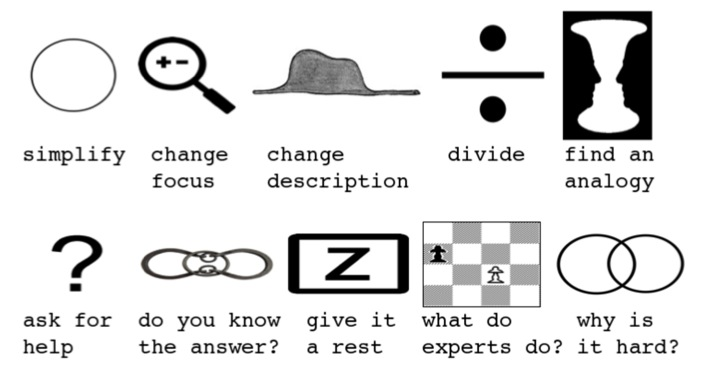
\includegraphics[width=\textwidth]{./pictures/heuristic-images.jpg}
\caption{Minskian heuristics for problem solving}
\end{figure}

We can see some relationships to the peeragogy patterns we've
identified, first summed up with a picture here, and in text below (some
of the nodes in the diagram are clickable, and clicking will take you to
the page describing that pattern!):

To elaborate in words:

- We \emph{simplify} things for a \textbf{Newcomer}. (In particular,
this means that we don't expect the newcomer to use a high processing
level.)

- We \emph{change focus} by using a \textbf{Roadmap} to guide us from
one step to another. In addition, the project's \textbf{Heartbeat} leads
us to let go of our focus at one moment, and resume with another point
of view later.

- We \emph{change description} first of all by having a \textbf{Wrapper}
who describes the new state of the project. For the Peeragogy project,
that often meant summing up the high points that we saw over a given
period of time. It seems possible that with a rich enough
\textbf{Pattern Language}, the description would itself be made in terms
of patterns.

- We \emph{divide} work up not only ``horizontally'' among different
\textbf{Roles}, but also ``temporally'' by using the \textbf{Roadmap}.
Someone who is moving ahead with the Roadmap is likely to be ``working
at the cutting edge''.

- When we \emph{find an analogy}, we are basically \textbf{Creating a
Guide} of some sort. This can be used as a form of ``exploration'', as
we look at how one form of engagement may or may not map onto other
forms of engagement.

- When we \emph{ask for help}, we may avail ourselves of some
\textbf{Moderation} service that will decide how to deal with our
request. One simple way to ask for help is \textbf{Polling for Ideas}.
Obviously once we start to get help, we're working in a regime of
``collaborative effort''.

- If you \emph{know the answer}, then you may be able to reuse it (which
is the basic idea described in \textbf{Praxis vs Poesis}, though the
title is a little bit obscure). Someone who knows the answer and who is
good at self-explanation may also have a good idea about how to get from
the current state to the goal state; alternatively, this may be broken
down into steps in some sub-Roadmap, and moving from step to step would
then illustrate ``progressive problem solving''.

- It is important to \emph{give it a rest} so as not to over-exhaust
oneself, busting one's own \textbf{Carrying Capacity}, or,
alternatively, overwhelming the group.

- It seems that one of the things that \emph{experts do} is
\textbf{Discerning a Pattern}. This allows them to simplify their
processing.

- Finally, again, if we \emph{know why it is hard}, then we may be able
to \textbf{Create a Guide} that will help get around, or at least better
cope with, the difficulty.
